\documentclass[]{spie}  %>>> use for US letter paper
%\documentclass[a4paper]{spie}  %>>> use this instead for A4 paper
%\documentclass[nocompress]{spie}  %>>> to avoid compression of citations

\renewcommand{\baselinestretch}{1.0} % Change to 1.65 for double spacing

\usepackage{amsmath,amsfonts,amssymb,gensymb}
\usepackage{graphicx}
\usepackage[colorlinks=true, allcolors=blue]{hyperref}
\usepackage{float}
\usepackage{lipsum}

% added by Austin Downey for editing		
\usepackage{color}
\usepackage{enumitem}
\usepackage{soul}
\newcommand{\bl}[1]{\textcolor[rgb]{0.00,0.00,1.00}{#1}}
\newcommand{\gr}[1]{\textcolor[rgb]{0.00,0.50,0.00}{#1}}
\newcommand{\rd}[1]{\textcolor[rgb]{0.75,0.00,0.00}{\st{#1}}}
\newcommand{\tl}[1]{\textcolor[rgb]{0,0.6,0.60}{#1}}	
\usepackage[textsize=tiny,textwidth=0.72in]{todonotes}	


\title{MLPUAV SPIE Paper}

\author[a]{Samuel Tadamatla} 
\author[a]{Evan Phillips} 
\author[b]{Md Asifuzzaman Khan}
\author[a,b]{Austin R.J. Downey}

\affil[a]{Department of Mechanical Engineering, University of South Carolina, Columbia, USA}

\authorinfo{Further author information: (Send correspondence to Austin Downey) \\Austin Downey: Email: austindowney@sc.edu}

% Option to view page numbers
%\pagestyle{plain} % change to \pagestyle{plain} for page numbers
%\setcounter{page}{1} % Set start page numbering at e.g. 301

\begin{document}
	\maketitle
	
	\begin{abstract}
		\lipsum[1-3]
	\end{abstract}
	
	% Include a list of keywords after the abstract
	\keywords{real-time monitoring, UAV-deployable, water quality, sensor nodes, wireless communication, open-source}
	
	
	\section{INTRODUCTION}
	\label{sec:intro}  % \label{} allows reference to this section
	
	\lipsum[1-5]
	
	\begin{figure}[h]
		\centering
		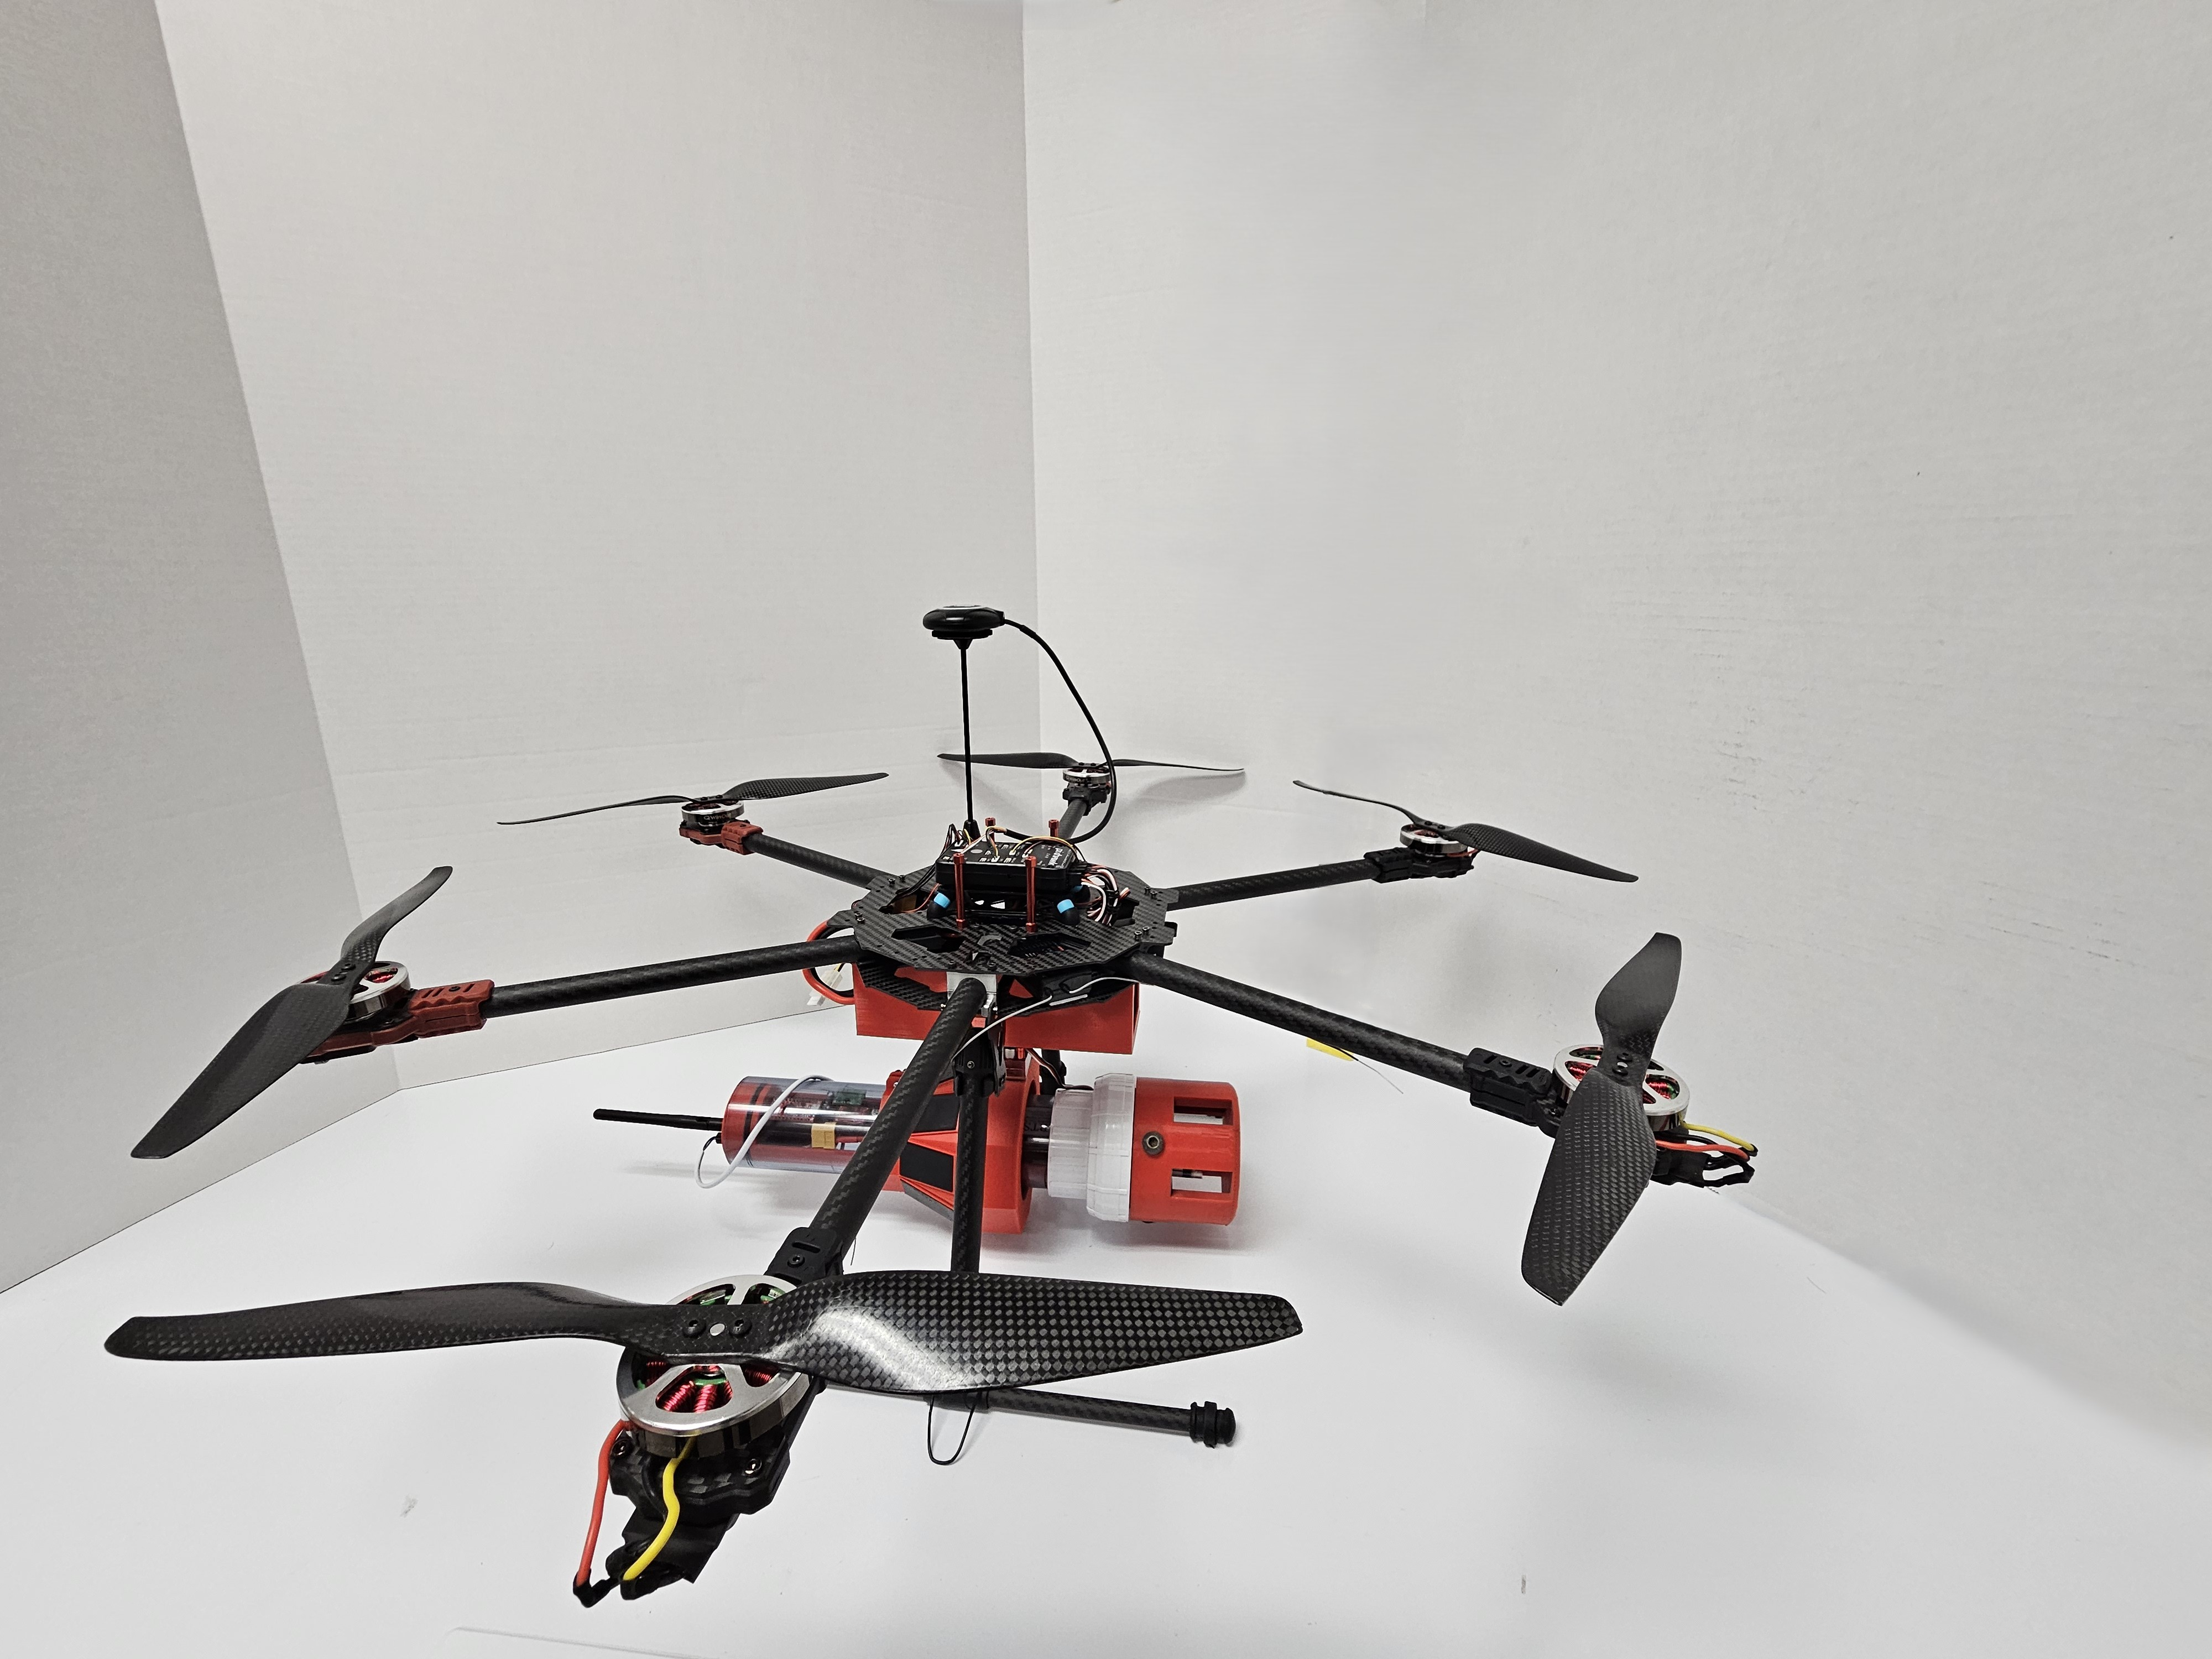
\includegraphics[width=0.9\textwidth]{figures/Figure1_Drone}
		\caption{Full drone setup showing main frame and propeller configuration.}
		\label{fig:Figure1_Drone}
	\end{figure}
	
	%\pagebreak
	\lipsum[1]
	
	\begin{figure}[h]
		\centering
		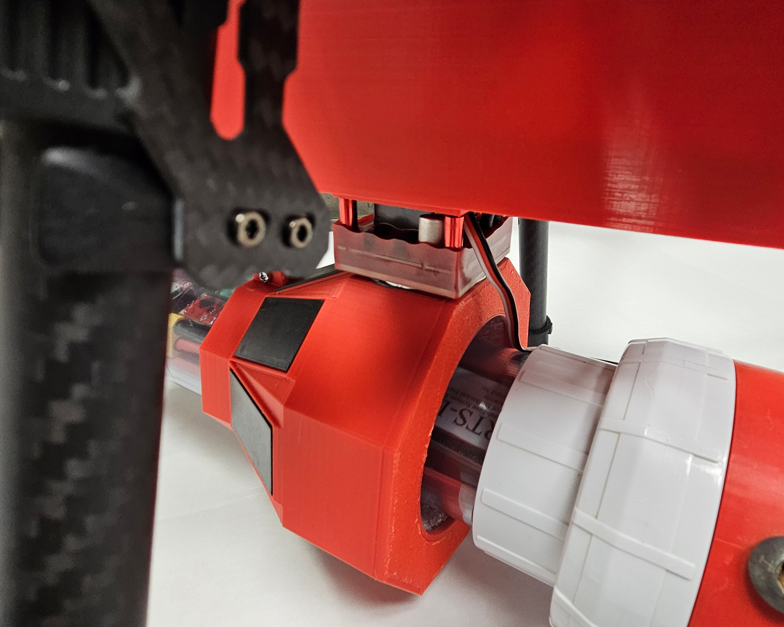
\includegraphics[width=0.9\textwidth]{figures/Figure2_EPM}
		\caption{Close-up of Electro-Permanent Magnet (EPM) attachment.}
		\label{fig:Figure2_EPM}
	\end{figure}
	
	\section{RESULTS}
	\label{sec:results}
	\lipsum[1-3]
	
	\begin{figure}[H]
		\centering
		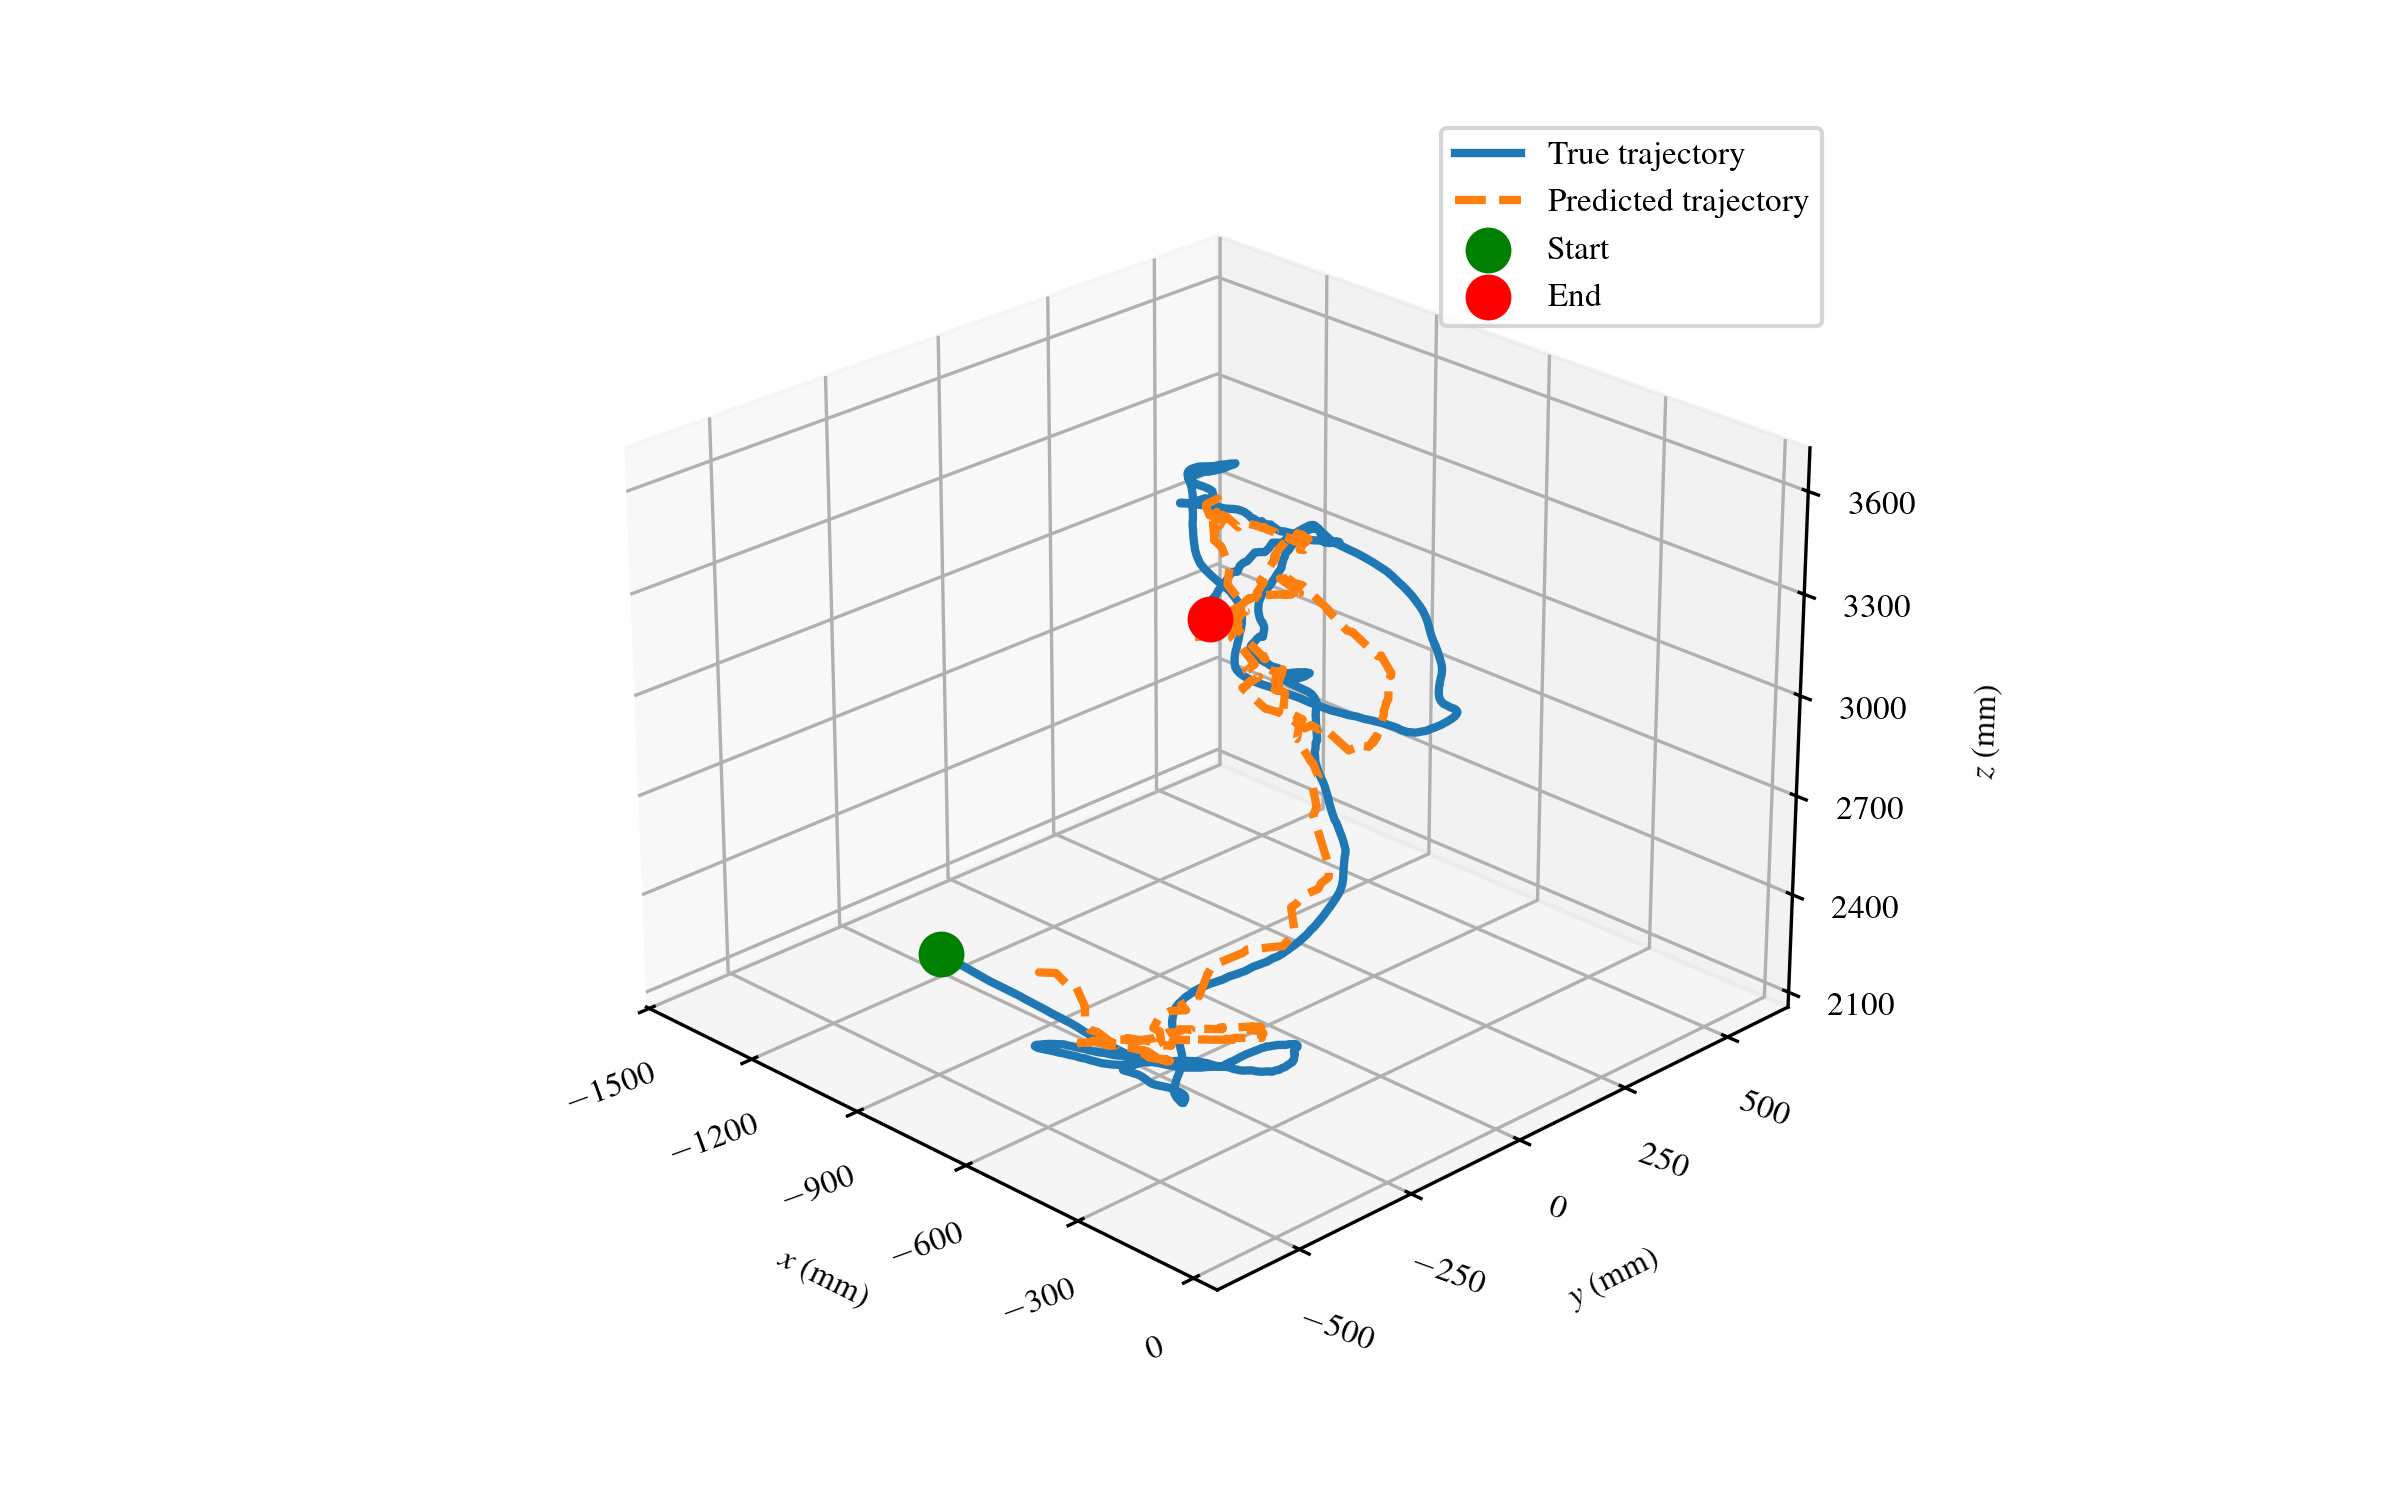
\includegraphics[width=8.0in]{figures/Figure3_3D_Trajectory}
		\caption{Comparison of the drone's 3D trajectory, showing predicted and true flight paths.}
		\label{fig:Figure3_3D_Trajectory}
	\end{figure}
	
	\lipsum[1]
	
	\begin{figure}[H]
		\centering
		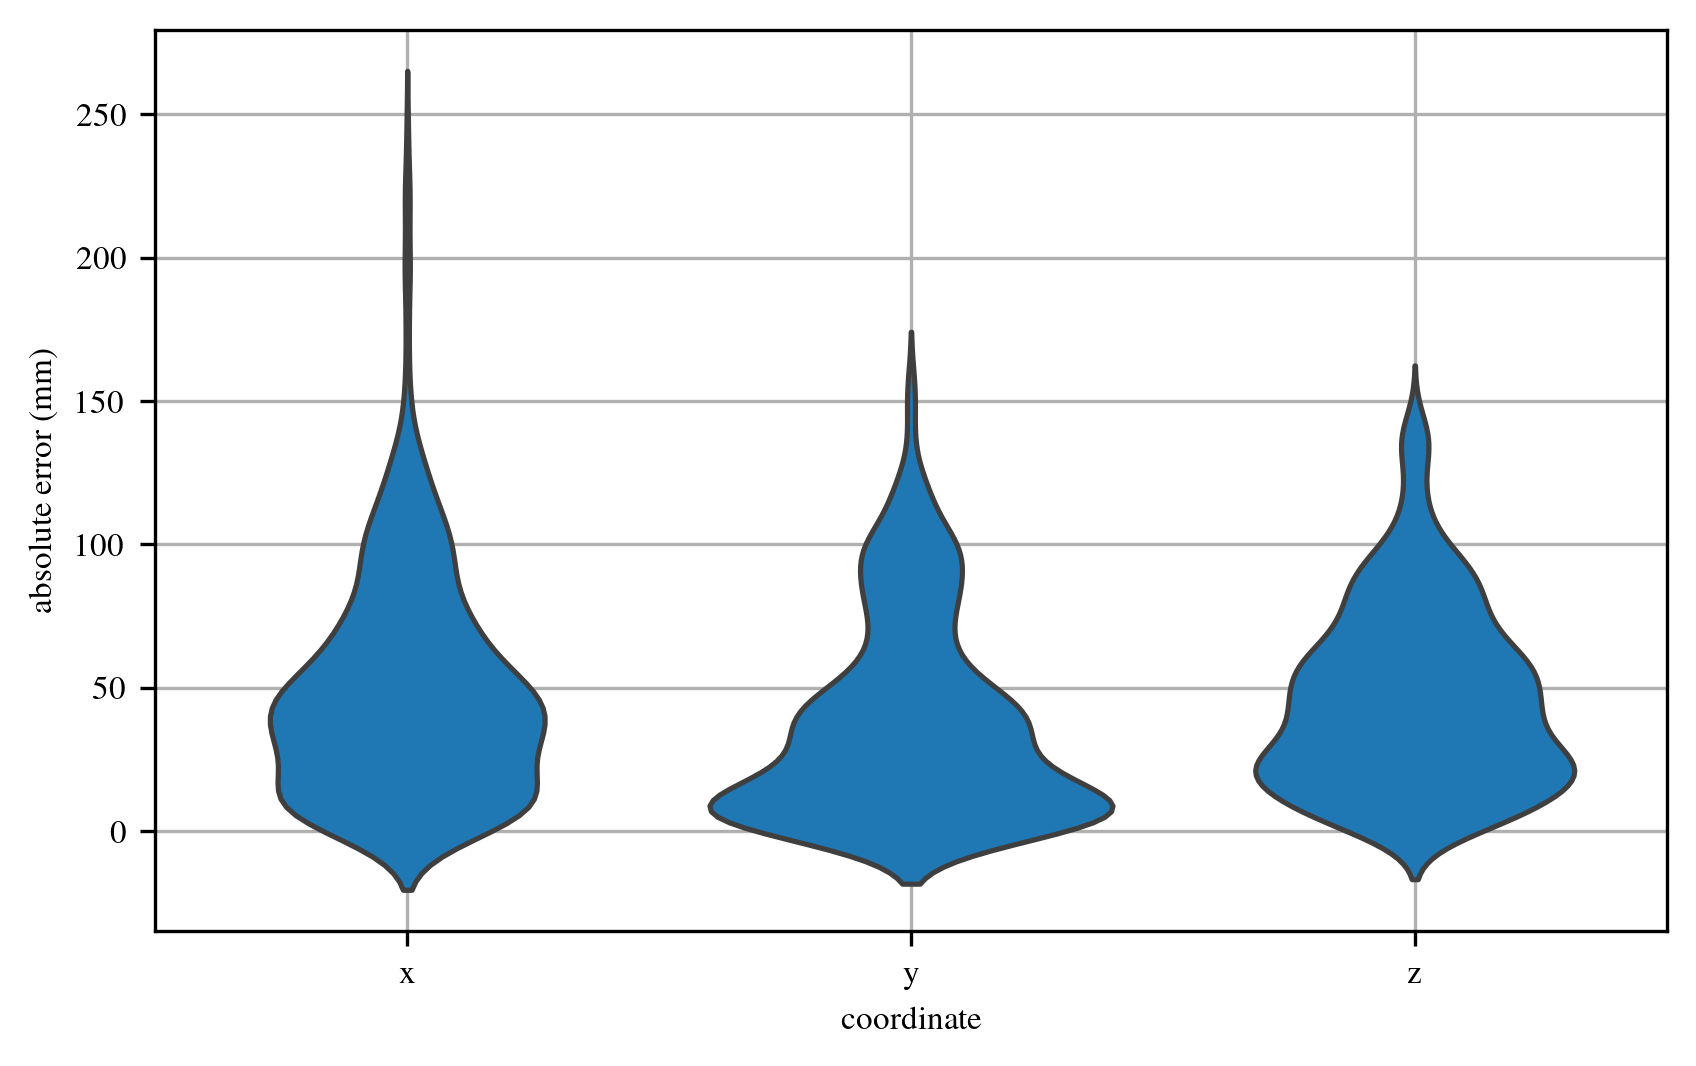
\includegraphics[width=6.5in]{figures/Figure4_Error_Distribution}
		\caption{Distribution of prediction errors for X, Y, and Z coordinates.}
		\label{fig:Figure4_Error_Distribution}
	\end{figure}
	
		\lipsum[1-2]
	
	\begin{figure}[H]
		\centering
		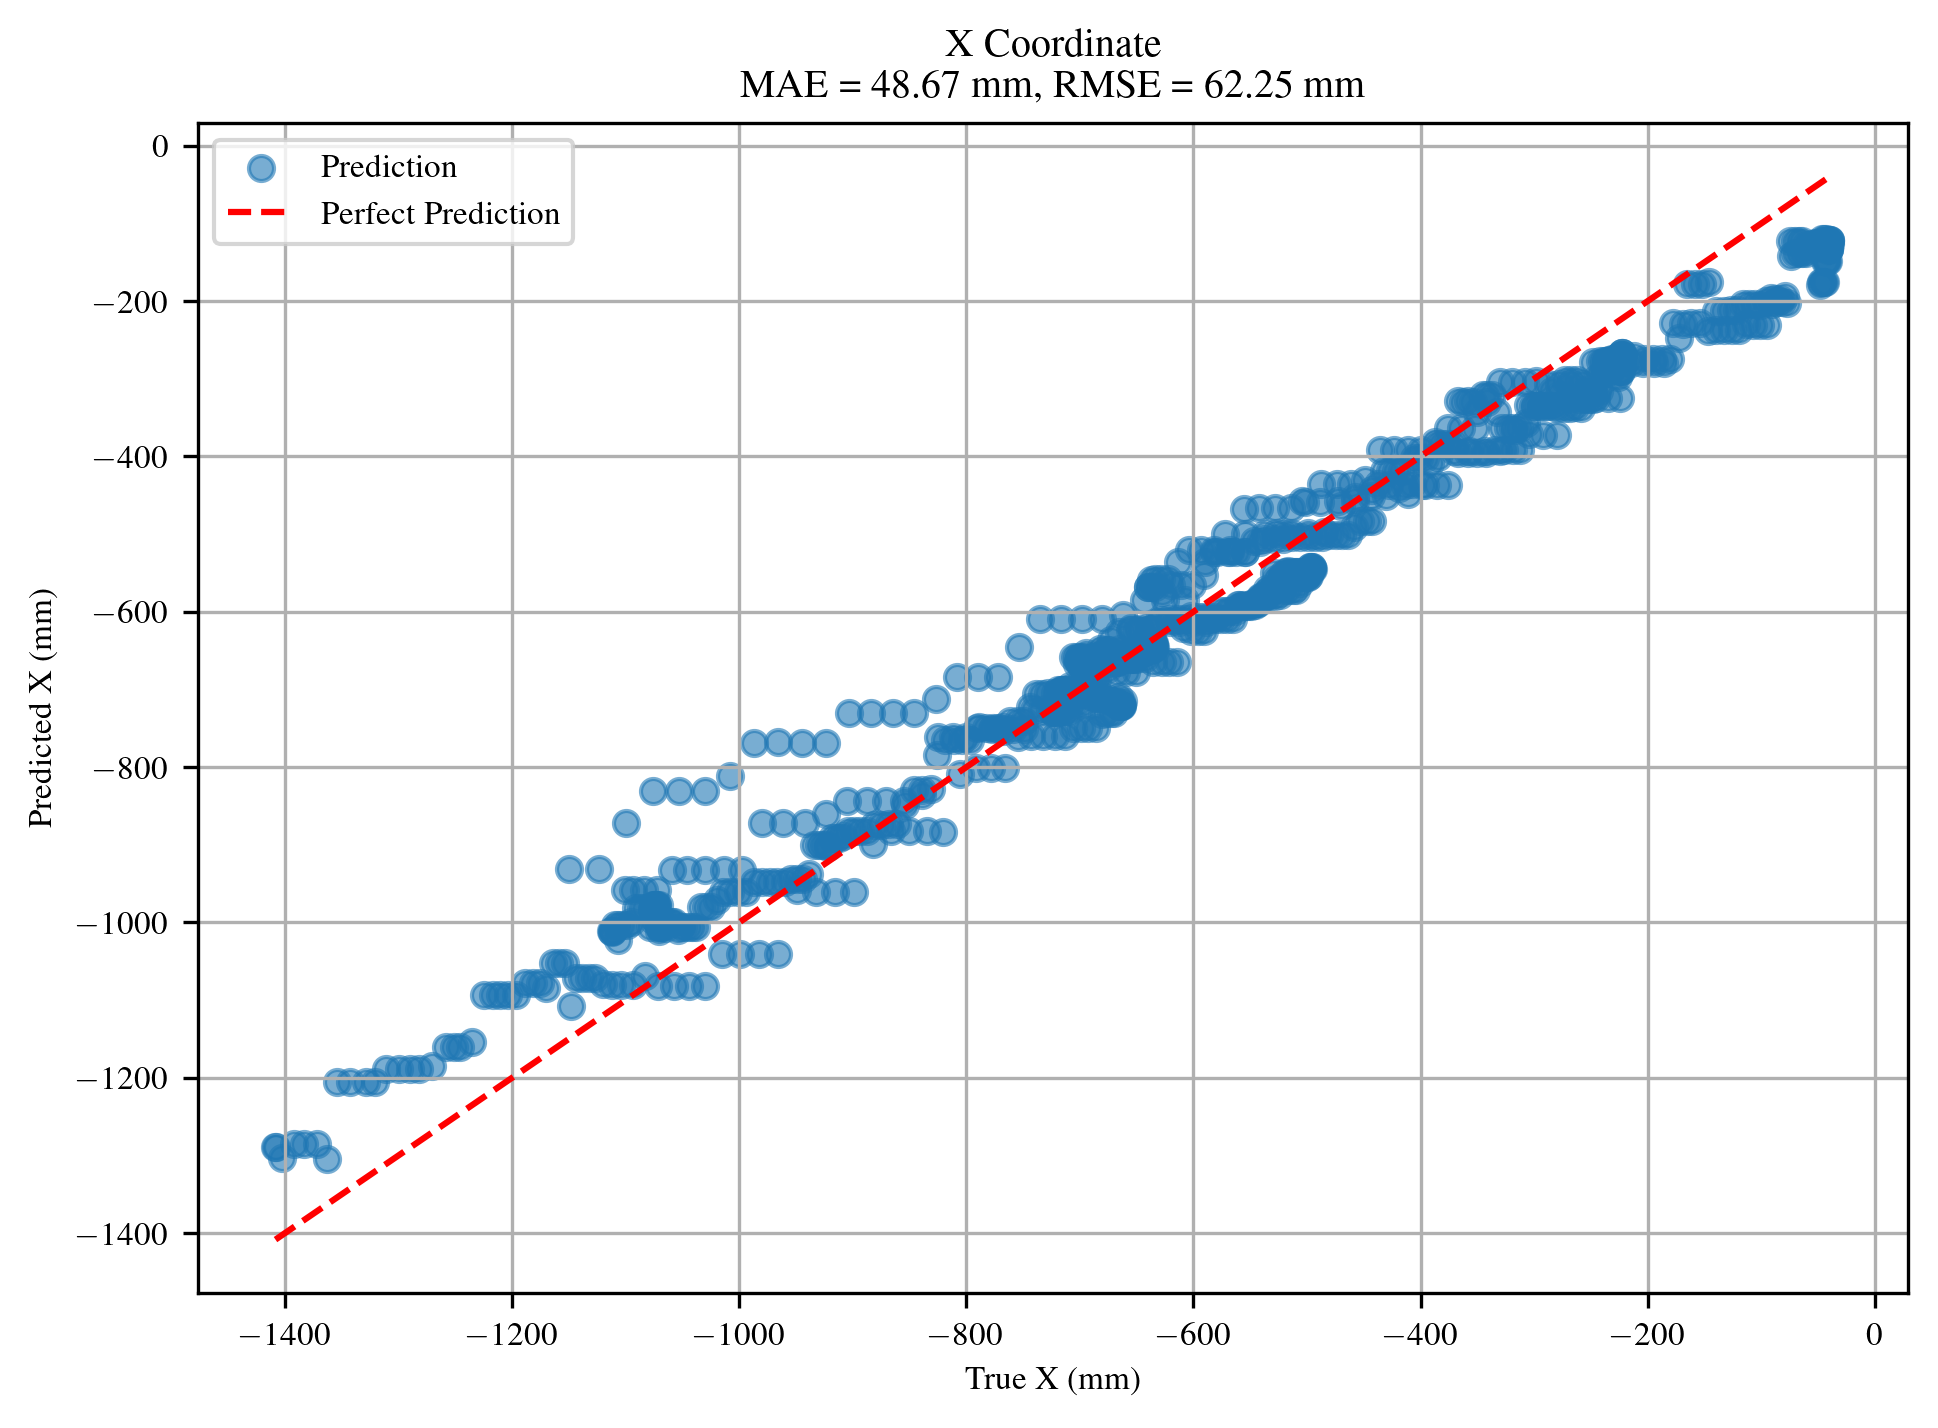
\includegraphics[width=6.5in]{figures/Figure5_Scatter_X}
		\caption{Scatter plots visualizing predicted versus true coordinates for X.}
		\label{fig:Figure5_Scatter_X}
	\end{figure}
	
	\begin{figure}[H]
		\centering
		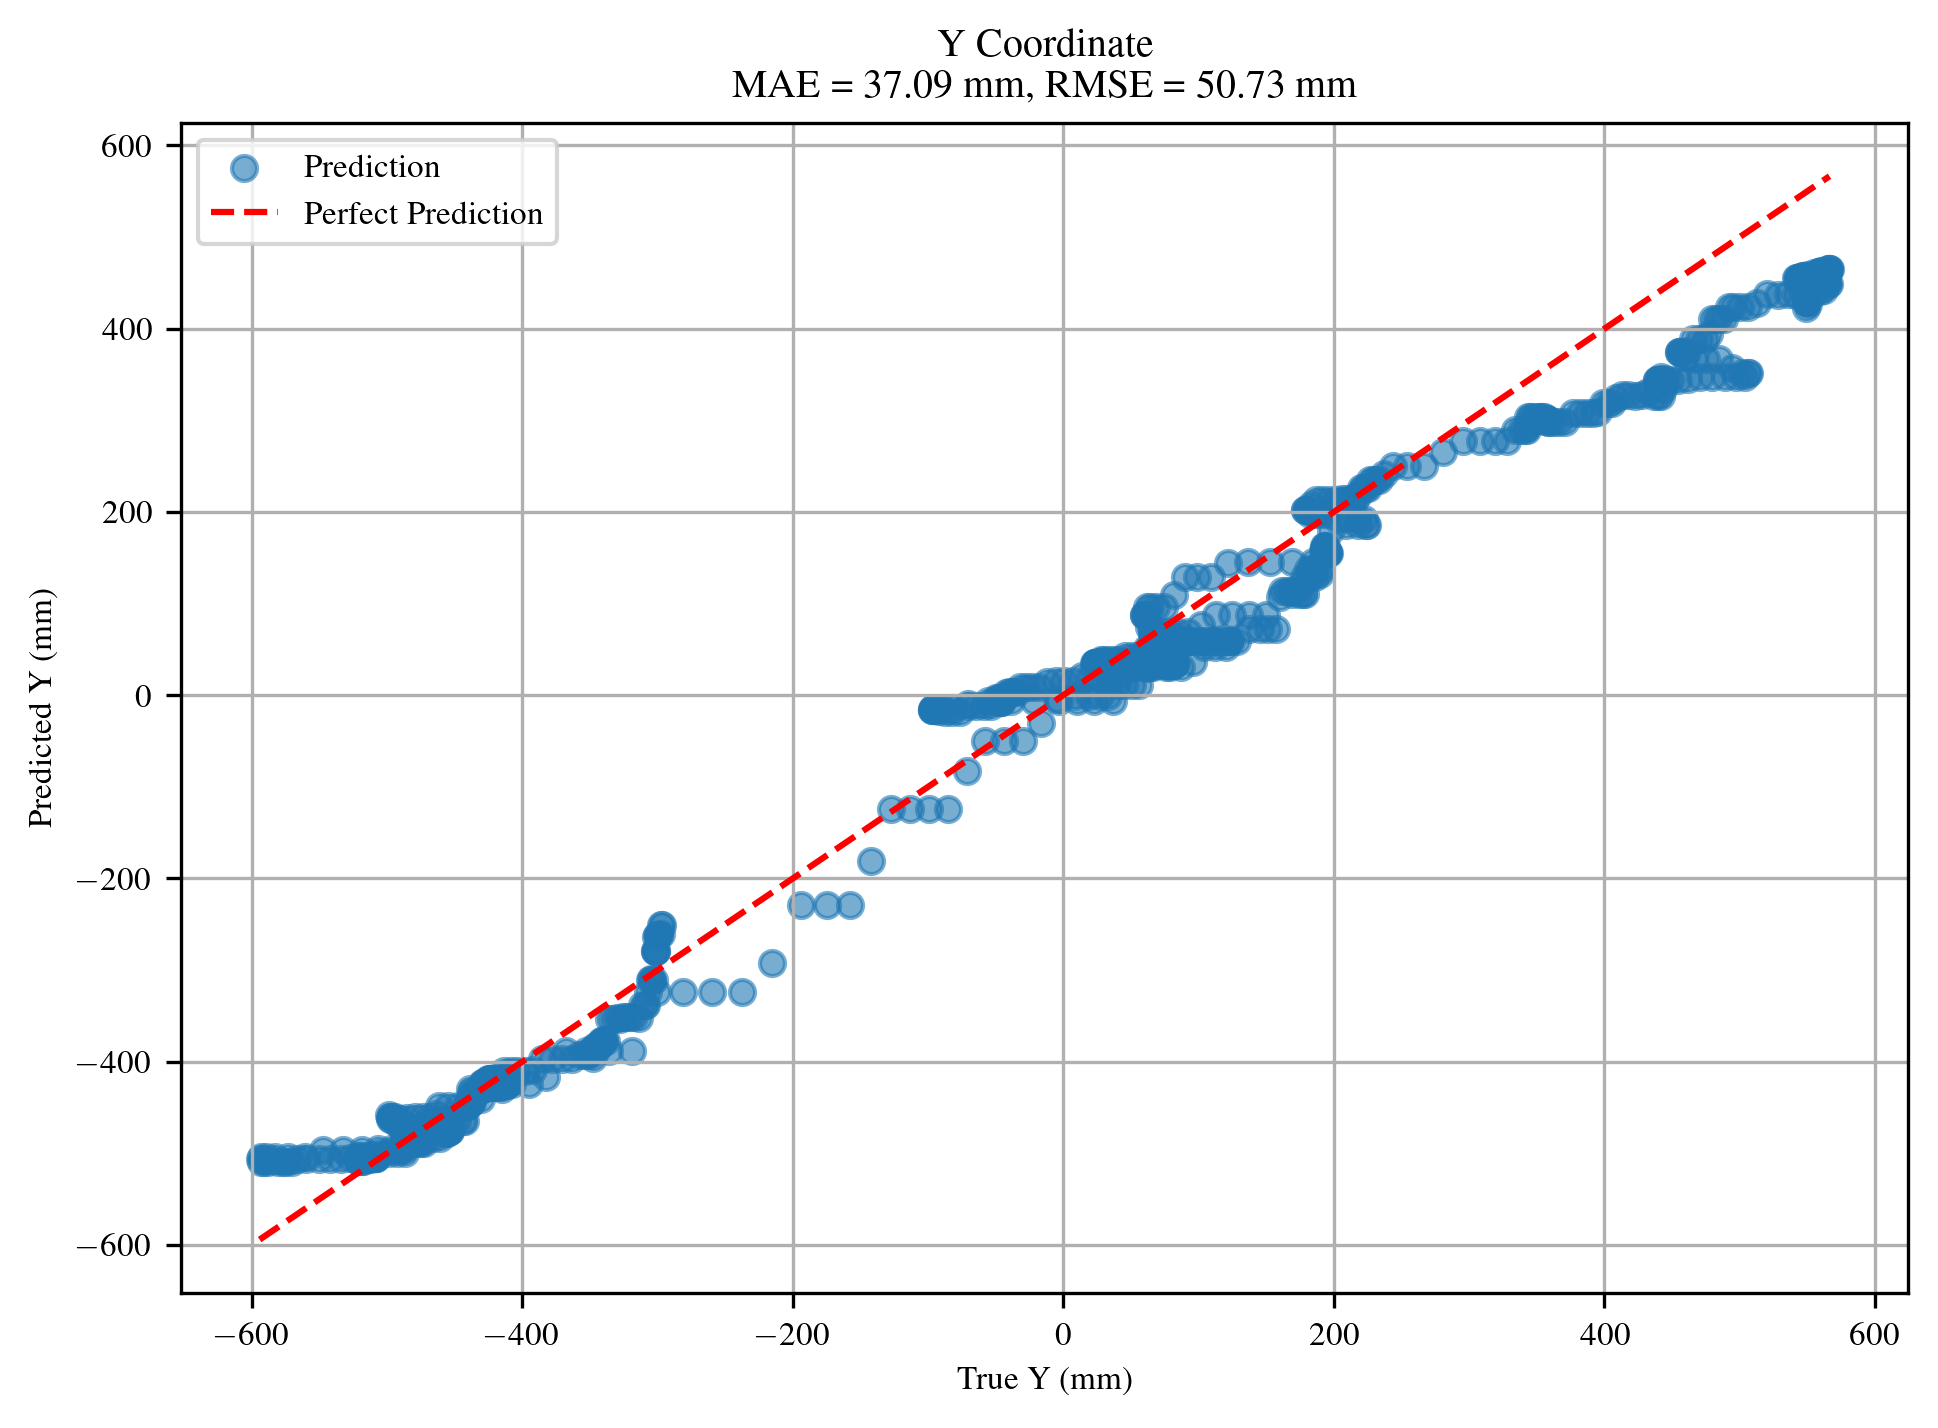
\includegraphics[width=6.5in]{figures/Figure5_Scatter_Y}
		\caption{Scatter plots visualizing predicted versus true coordinates for Y.}
		\label{fig:Figure5_Scatter_Y}
	\end{figure}
	
	\begin{figure}[H]
		\centering
		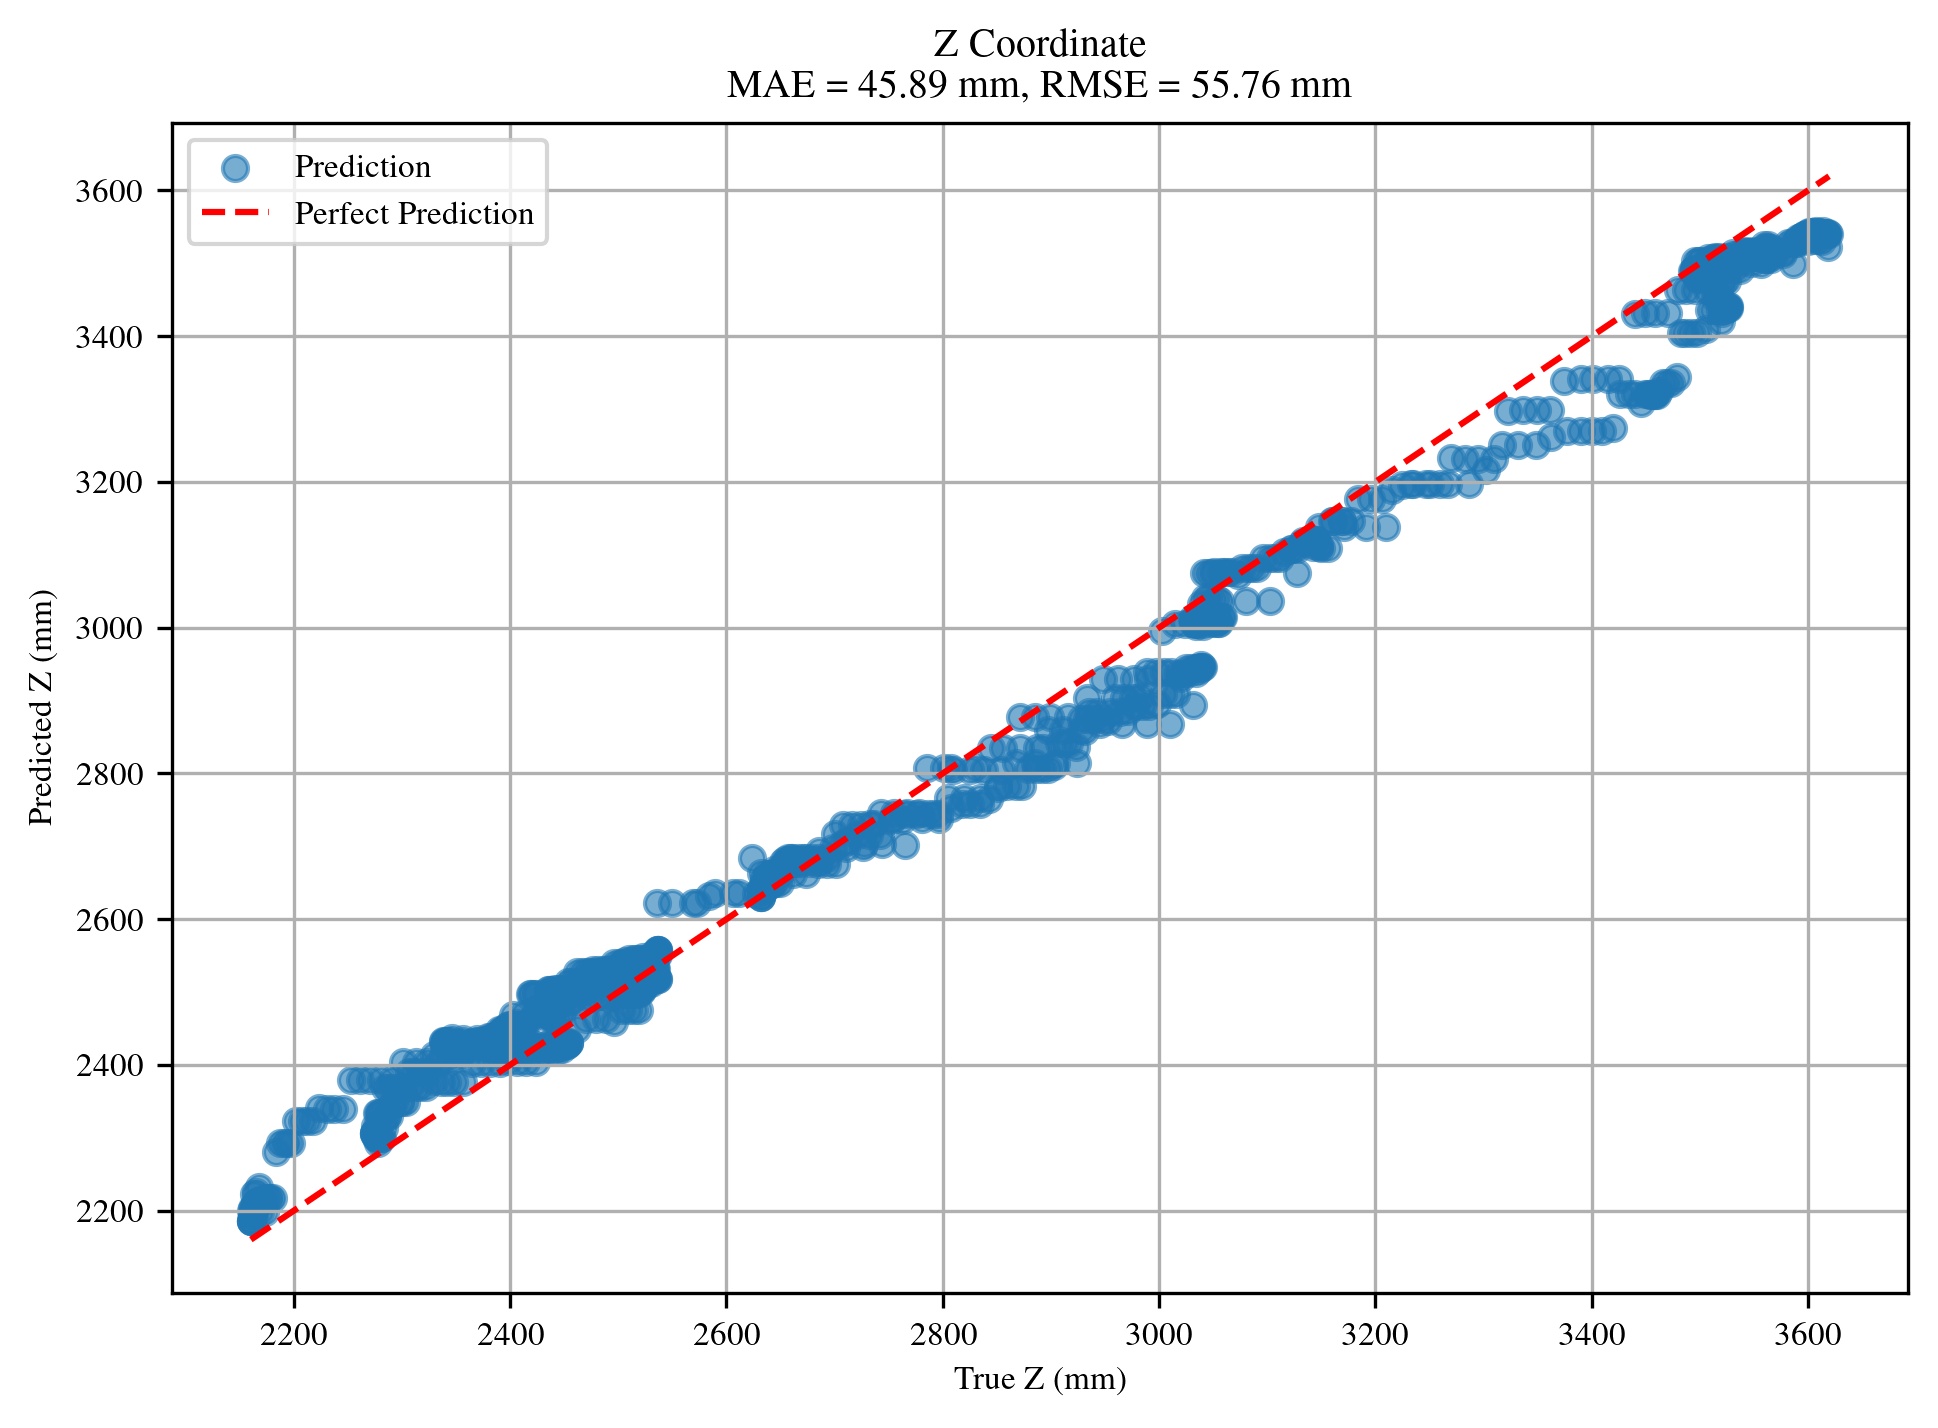
\includegraphics[width=6.5in]{figures/Figure5_Scatter_Z}
		\caption{Scatter plots visualizing predicted versus true coordinates for Z.}
		\label{fig:Figure5_Scatter_Z}
	\end{figure}
	
	\lipsum[1-2]
	
	\begin{figure}[H]
		\centering
		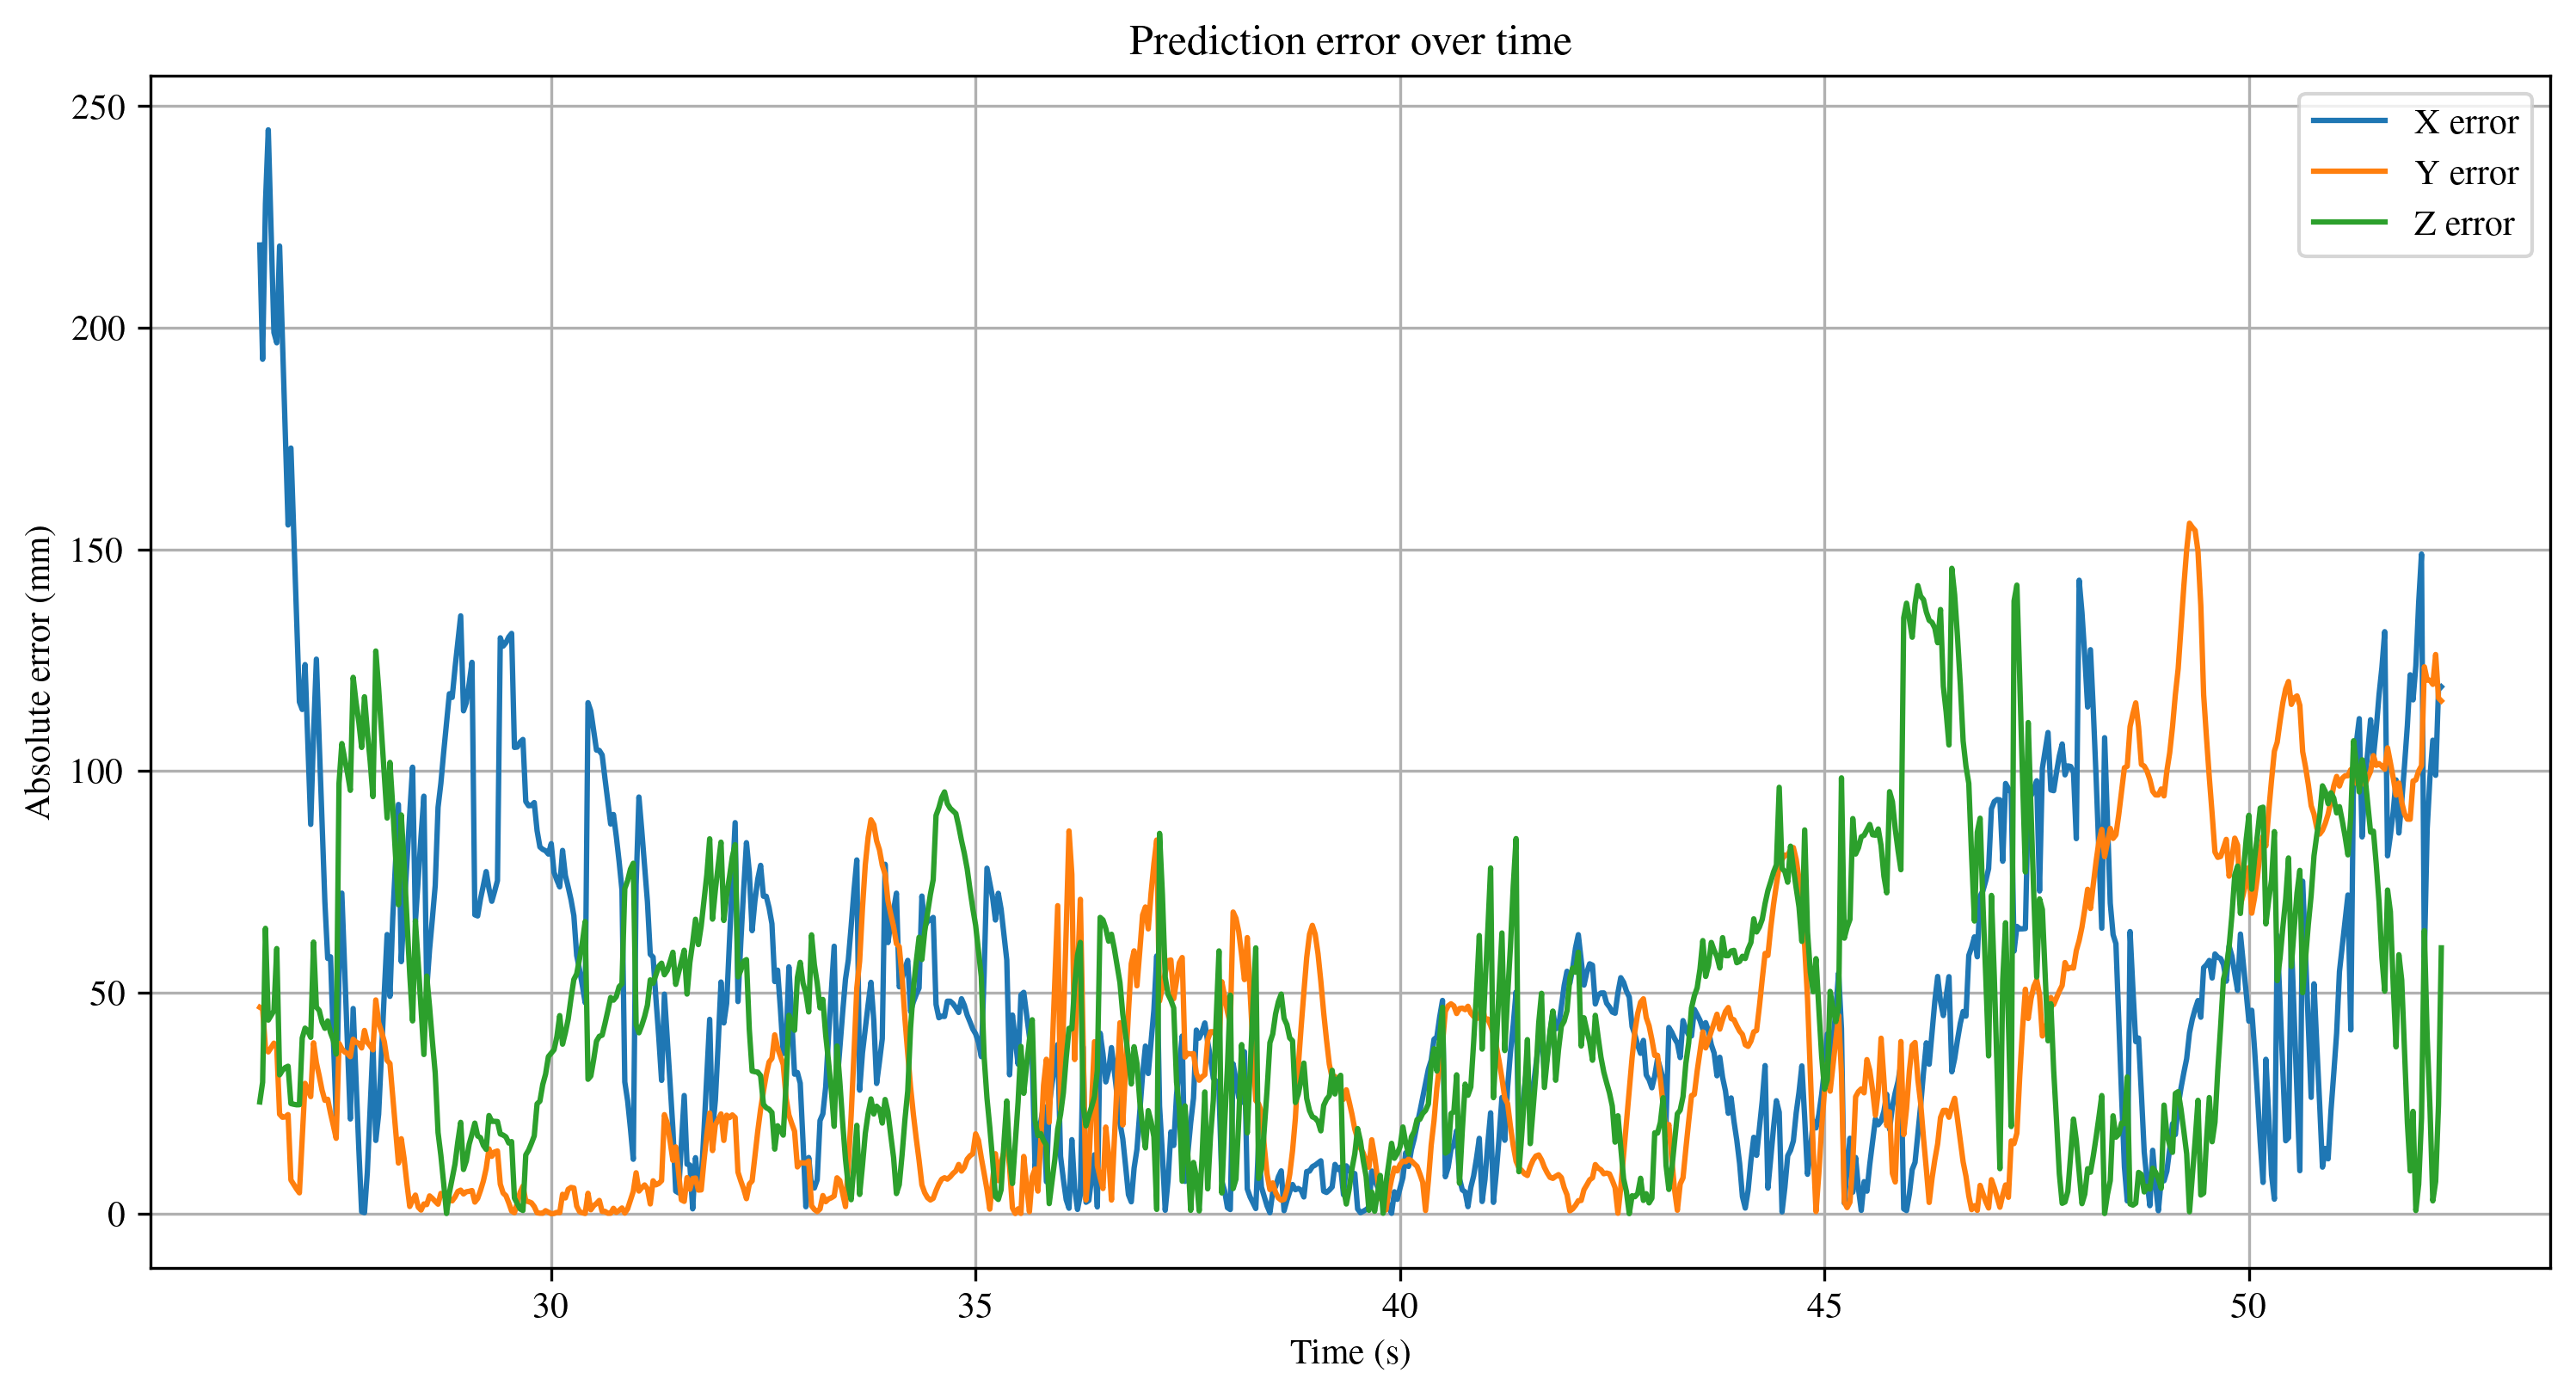
\includegraphics[width=6.5in]{figures/Figure6_Error_Over_Time}
		\caption{Prediction error visualized over time for each axis (X, Y, Z).}
		\label{fig:Figure6_Error_Over_Time}
	\end{figure}
	
	\lipsum[1-2]
	
	% References
	\bibliography{references} % bibliography data in report.bib
	\bibliographystyle{spiebib} % makes bibtex use spiebib.bst
	
\end{document}
